The correct execution can only be guaranteed as long as the integrity of the environment is ensured.
When circumventing the \gls{lvl} the code has to be modified.
Unless done precisely, this can be detected, e.g. \gls{luckypatcherg} does not have the developers signature and thus uses a different one.
Other breaches of integrity are debuggability and \textit{root}, cracking applications and unaurthorized installation.
In order to be able to detect this and prevent the execution of the application a priori, additional checks are implemented as seen in figure~\ref{fig:verificationNowAdditional}.
\begin{figure}[h]
    \centering
    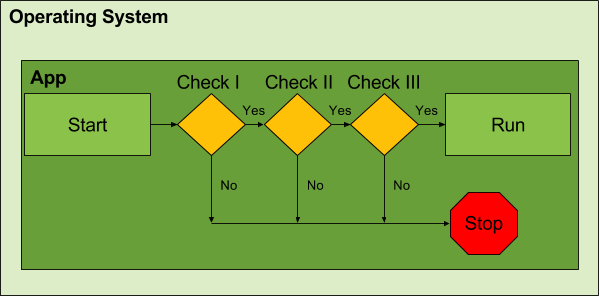
\includegraphics[width=0.8\textwidth]{data/verificationNowAdditional.png}
    \caption{Introduction of additional tests to check environment and integrity of the application}
    \label{fig:verificationNowAdditional}
\end{figure}
Since all tampering countermeasures have the same pattern in operation, they can be circumvented easily.
The goal of these checks is to increase the workload of an attacker since the code has to be analysed in order to find, understand and patch them.
In order to make this task even more time consuming, these checks can be obfuscated and spread inside the application.
Even the possibility of implementing them in native code can be considered.
\newline
This does not prevent \gls{luckypatcherg} itself from working, but it offers an additional layer of security which has to be voided.
